\documentclass[journal, letterpaper]{IEEEtran}
%\documentclass{scrartcl}

\usepackage[english]{babel}
%\usepackage[latin1]{inputenc}
\usepackage[utf8]{inputenc}
\usepackage[T1]{fontenc}
\usepackage{amsmath}
\usepackage{amsthm}
\usepackage{amsfonts}
\usepackage{tikz}
\usepackage{verbatim}
\usepackage{subcaption}
\usepackage{algorithm}
\usepackage{algorithmic}
\usepackage[pdftex]{hyperref}

\renewcommand{\algorithmicrequire}{\textbf{Input:}}
\renewcommand{\algorithmiccomment}[1]{\ \ // #1} % C-like // Comments

\hyphenation{render}

% No clubs and widows allowed
\clubpenalty10000
\widowpenalty10000
\displaywidowpenalty=10000
\DeclareMathOperator*{\argmin}{arg\,min}
\begin{document}

%\title{Simulating elastic spheres without external forces}
%\subtitle{Project 1 for class CS6491 Computer Graphics}
\title{Curve Average \\
	{\large Project 3 for class CS6491 Computer Graphics}}
%\author{Sebastian Weiss}
\author{Sebastian Weiss, Can Erdogan \\ \today}
%\date{\today}

\maketitle

\begin{tikzpicture}[remember picture,overlay]
   \node[anchor=north east,inner sep=0pt] at (current page.north east)
              {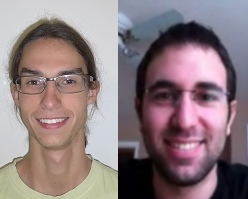
\includegraphics[scale=1.5]{pic}};
\end{tikzpicture}

\section{Objective}
Formally, for two curves $A = \{a_0 ... a_{n-1}\}$ and $B = \{b_0 ... b_{n-1}\}$, each with $n$ points and $\forall x \in (A \cup B), x \in \mathcal{R}^3$,
the goal is to find a curve $C$ such that for each point $c \in C$, and its closest projections
\begin{align}
a^c &= \operatornamewithlimits{argmin}\limits_{a \in A} ||a-c|| \text{, and} \\
b^c &= \operatornamewithlimits{argmin}\limits_{b \in B} ||b-c||
\end{align}

\noindent the following holds true:

\begin{equation}
 c = \operatornamewithlimits{argmin}\limits_{x \in L(a^c, b^c)} ||a^c-x||
\end{equation}

\noindent where for each point $r$ on line $L(p,q)$, $||r-p|| = ||r-q||$. Moreover, for
any three consecutive sampled points $c_i$, $c_j$ and $c_k$ on curve $C$, the arc lengths
of the curves between their closest projections are the same:
\begin{equation}
\small
 D^A(a^{c_i},a^{c_j}) + D^B(b^{c_i},b^{c_j}) = D^A(a^{c_j},a^{c_k}) + D^B(b^{c_j},b^{c_k})
\end{equation}
\noindent where $D^Z(x,y)$ is the distance along the curve $Z$ between points $x,y \in Z$.

Semantically, we want to find the curve that is composed of the loci of the smallest spheres that touch the two inputs curves A and B,
and sample it such that for each sample on the curve, the distances traveled by the matching samples along their curves is a constant.

\section{Input}
The input is the six control points for two curves $A$ and $B$ such that the first and the last control points are the same.

\section{Overview}
The project is composed of the following three main parts: (1) the representation of the curves,
(2) the computation of the average curve, and (3) the visualization of the different curve properties.
The challenge in the representation is that we want the spline curves to first meet at two end points and then,
to have $C^1$ continuity at the intersection of the splines. For the curve average, we had to ensure
the points satisfied the constraints in Equations 1-3. Lastly, the visualization contained multiple challenges
including parallel transport, circular arc computation and etc.

\section{Curve Representation}

\subsection{Quadratic Hermite Spline}
\subsection{Cubic Hermite Spline}

\section{Average Curve Computation}

\subsection{Distance functions}
\subsection{Average Distance Sampling}

\section{Visualization Algorithms}

\section{Results}

\section{Future work}

\end{document}